% !TeX spellcheck = en_US

%Schriftgröße, Layout, Papierformat, Art des Dokumentes
\documentclass[10pt,oneside,a4paper]{article}

%Einstellungen der Seitenränder
\usepackage[left=3cm,right=4cm,top=3cm,bottom=6cm,includeheadfoot]{geometry}

%Umlaute ermöglichen
\usepackage[utf8]{inputenc}
%\usepackage[ngerman]{babel}
\usepackage{url}
\usepackage{graphicx}
\usepackage{subfigure}
\usepackage{float}
\usepackage{hyperref} % important: load after float
\hypersetup{
	pdftitle={CoreASM Editor \& Debugger --- Manual},
	pdfauthor={Marcel Dausend},
	pdfsubject={CoreASM Editor \& Debugger --- Manual},
	pdfproducer={pdfeTex 3.14159-1.30.6-2.2},
	colorlinks=false,
	pdfborder=0 0 0	% keine Box um die Links!
}

%Kopf- und Fußzeile
\usepackage{fancyhdr}
\pagestyle{fancy}
\fancyhf{}

%Kopfzeile links bzw. innen
\fancyhead[L]{\thepage}
%Kopfzeile rechts bzw. außen
\fancyhead[R]{\nouppercase{\leftmark}}
%Linie oben
\renewcommand{\headrulewidth}{0.5pt}
%Linie unten
\renewcommand{\footrulewidth}{0.5pt}
\newcommand{\copyrightNotice}[1]{{\small Copyright \copyright\ #1}}
%\newcommand{\revision}{{\footnotesize Document \mbox{$Revision: #27 $}}}


\usepackage{listings}
\lstset{
numbers=left,
stepnumber=1,
numbersep=5pt,
numberstyle=\small\color{black},
basicstyle=\ttfamily,
commentstyle=\itshape,
morecomment=[l]{//},
morecomment=[s]{/*}{*/}
}

\usepackage[os=win]{menukeys}
%\renewmenumacro{\menu}[>]{menus}
\newmenumacro{\mydirectory}[/]{hyphenatepathswithfolder}
\renewmenumacro{\mykeys}[+]{roundedkeys}


\begin{document}
\title{
	CoreASM Editor \& Debugger --- Manual
	\vspace{.5cm}\\
	\huge An advanced Editor and Debugger\\for CoreASM\\%\\ {\Large Version }
	\vspace{.5cm}
	\normalsize
	\url{http://uni-ulm.de/in/pm/projects/coreasm}\\
	\url{https://github.com/CoreASM/}\\
	\url{http://coreasm.org}
}

\author{Marcel Dausend, Markus Müller, and Michael Stegmaier\\ \ttfamily \small \{marcel.dausend, markus.mueller, michael-1.stegmaier\}@uni-ulm.de}
\date{Version 1.7.0-SNAPSHOT, March 2013}% \\ \revision}

\maketitle
\vfill
\section{Introducing Notes}
The CoreASM Eclipse plugin extends the Eclipse IDE for editing, debugging, and executing CoreASM specifications. This version is a major upgrade from the latest version (0.6.8.beta). It offers a reimplemented and enhanced editor which integrates the latest jparsec parser\footnote{\url{http://jparsec.codehaus.org/}}. This new editor performs noticeably better than the old one and introduces some valuable features to revise specifications like quick fixes and syntax checks. Furthermore, CoreASM specifications can be investigated in an intuitive as well as comprehensive manner with the new debugger which makes use of the regular Eclipse debugging components.

The reimplementation and enhancement of the editor component has been implemented by Markus Müller during his diploma thesis \cite{Mueller2012}. The debugger has been implemented as part of a bachelor thesis by Michael Stegmaier \cite{Stegmaier2012} and has been introduced on the ABZ-conference 2012 in Pisa \cite{Dausend.Stegmaier.ea2012}. Both theses have been supervised by Prof. Dr. Helmuth A. Partsch, head of the institute of Software Engineering and Compiler Construction at the University of Ulm. The work has been initiated and mentored by Marcel Dausend. Meanwhile, the project has been merged with the official CoreASM development project (\url{www.coreasm.org}) and is provided as open source via github \cite{Dausend.Farahbod.ea2012}.

\newpage
% %table of contents
\tableofcontents
\newpage


\section{The CoreASM Eclipse Plugin}
The daily version of the CoreASM Eclipse plugin can be received via github \cite{Dausend.Farahbod.ea2012}. A guide for building and executing the development version can be found on the referred website, too. Non-developers can easily try out the latest release version of the CoreASM Eclipse plugin by themselves.  It is distributed via the \href{https://marketplace.eclipse.org/content/coreasm-eclipse-plugin}{Eclipse Marketplace} and our \href{http://webcoreasm.informatik.uni-ulm.de/coreasm-repository/}{Eclipse Update Site}. Further information can be found in our \href{https://github.com/CoreASM/coreasm.core/wiki}{wiki at github}. You are welcome to contact the authors in case of questions or for providing your feedback\footnote{please send a request by e-mail to \url{marcel.dausend@uni-ulm.de}}.

\subsection{System Requirements}
The following infrastructure is required for the CoreASM Eclipse plugin:
\begin{itemize}
	\item Java SE Runtime Environment 7\\\url{http://www.oracle.com/technetwork/java/javase/downloads/index.html}
	\item Eclipse IDE for Java Developers (version \emph{Kepler} suggested)\\\url{http://www.eclipse.org/downloads/}
\end{itemize}

\noindent This version of the CoreASM Eclipse Plugin has been developed and tested under
\begin{table}[h]
\begin{tabular}{l}
	\begin{tabular}[c]{@{}l@{}}Ubuntu Linux 64bit v14.10 \&\\ Windows 7 and 8.1\end{tabular}\\
	\textit{with}\\
	\begin{tabular}[c]{@{}l@{}}Kepler Service Release 2 64 bit \&\\ Luna Eclipse Standard 4.4 64 bit\end{tabular}\\
	Oracle Java SE JDK 7
\end{tabular}
\end{table}

\subsection{Installing CoreASM Eclipse Plugin}

The Plugin can be installed either from the Eclipse Marketplace or by performing the following steps:

\begin{itemize}
\item Check if the required software (see above) is already installed on the target machine and if not, install the software.
\item Open the \menu{Help}-menu inside Eclipse
\item Select the menu item \menu[,]{Help, Install New Software...}
\item Paste the url of this site \url{http://webcoreasm.informatik.uni-ulm.de/coreasm-repository} into the field "work with" and press \keys{ENTER}
\item Next press \keys{Select All}- and afterwards \keys{Next}-button
\item Confirm the selection of the "CoreASM Eclipse Plugin" for installation by pressing the \keys{Next}-button
\item Accept the license and start the installation by pressing the \keys{Finish}-button
\item When the warning appears that you are installing unsigned content, you have to press the \keys{Okay}-button to continue
\item Last, you have to restart Eclipse so that the "CoreASM Eclipse Plugin" becomes available to you
\end{itemize}

If you like, you can build CoreASM by your own using the sources on github. The sources and our wiki are available at \url{https://github.com/CoreASM/coreasm.core}.


\section{General Introduction to CoreASM and its Editor}
The CoreASM plugin for Eclipse offers two components which are designed to support writing CoreASM specifications: The redesigned editor (see fig.\,\ref{fig:editor} -- middle) and an outline view of the currently open CoreASM specification (see fig.\,\ref{fig:editor} -- right).
Moreover, a view showing the AST of the current specification is provided to assist, for instance, in plug-in development.

\begin{figure}[h]
\centering
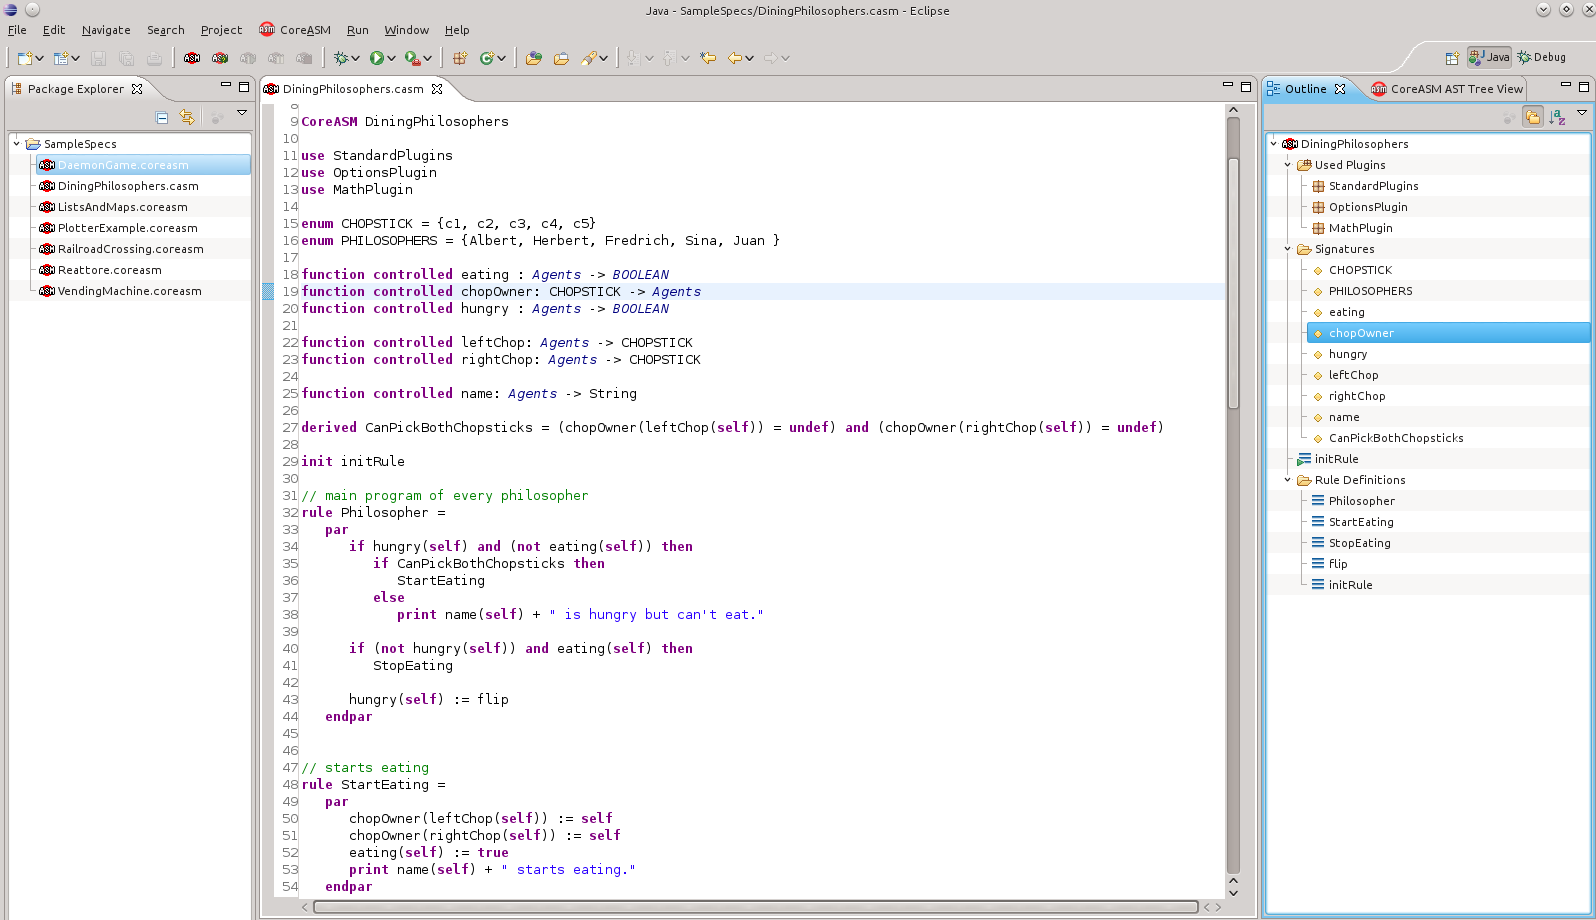
\includegraphics[width=\textwidth]{images/editor.png}
\caption{Overview of the Eclipse IDE, showing the CoreASM editor and its outline view}
\label{fig:editor}
\end{figure}


The editor offers a lot of features to support the user to create, examine, and correct or revise specifications:
\begin{itemize}
	\item syntax highlighting
	\item syntax checking
	\item warning and error markers (which are also shown in the eclipse problems view)
	\item quick fixes for several issues
	\item tooltips showing parser information
	\item bracket highlighting
	\item code completion
	\item \ldots
\end{itemize}

The outline view shows an overview of the specification corresponding to the currently open editor. The user can decide if the entries should be shown in a structured way, where use-statements, signatures and rules are grouped or in a flat representation. Also, the user can decide if the entries should be ordered alphabetically or in textual order of the specification. The buttons at the top of the outline view can be used to toggle between those configurations. Moreover, entries in the outline view can be used to navigate to their corresponding definition inside the specification by simply clicking on the desired entry. If the current specification cannot be parsed correctly, the outline view is marked as outdated. In this case, the user is advised to correct the specification before he can continue to use the outline view.

\subsection{Creating a Specification}
To create a CoreASM specification, an existing project in the current eclipse workspace is required as a container for the new specification. A new project can be created in three steps:
\begin{enumerate}
	\item Choose \menu{\underline{F}ile > \underline{N}ew > P\underline{r}oject\ldots} from the Eclipse menu or press \keys{\ctrl + N}.
	\item Choose \menu{General > Project} from the \emph{New Project} dialog.
	\item Give the new project a name and press \keys{\enter} or click on the \emph{Finish}-button.
\end{enumerate}

A CoreASM specification can be created in at least two ways: One way is creating a new text file with a name ending on \mydirectory{.casm} or \mydirectory{.coreasm} within the project of choice. An alternative is the \emph{new}-wizard:
\begin{enumerate}
	\item Choose \menu{\underline{F}ile > \underline{N}ew > \underline{O}thers\ldots} from the Eclipse menu or press \keys{\ctrl + N}.
	\item In the appearing \emph{New}-dialog select \menu{CoreASM > CoreASM Specification} and press \keys{\enter} or click on the \emph{Next}-button.
	\item Preferably select a project from the workspace as a container for the specification. This can be done by either using the file selection dialog or manually entering the project's name.
	\item Give the new specification file a name ending with \mydirectory{.casm} or \mydirectory{.coreasm} and press \keys{\enter} or click on the \emph{Finish}-button.
\end{enumerate}

The structure of a CoreASM specification and the CoreASM language are described in ``CoreASM Language User Manual''~\cite[p.\,7]{Rarahbod2011}\footnote{\url{http://coreasm.svn.sourceforge.net/viewvc/coreasm/engine-carma/trunk/doc/user\_manual/CoreASM-UserManual.pdf}}. A ``Hello World!''-example is given in section~\ref{ch:hello-world}.

\subsection{Executing a Specification}
A CoreASM specification can be executed using Carma \cite[p.\,4]{Rarahbod2011}\footnote{Carma can be received at \url{www.coreasm.org/download}} or the CoreASM Eclipse plugin. There are two ways to execute a CoreASM specification in Eclipse:

The easiest way to run the specification of the currently selected editor component is to click on the green run-button 
\includegraphics[height=.8em]{images/run-button.png} of the eclipse toolbar (see fig.\,\ref{fig:toolbar} and fig.\,\ref{fig:runningASpec}). As a result, the selected specification is executed by the CoreASM engine and the output is shown inside the \emph{Console}-view of Eclipse (see fig.\,\ref{fig:output}).
\begin{figure}[h]
\centering

\subfigure[Relevant excerpt of the Eclipse tool bar]{
	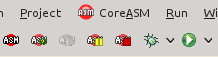
\includegraphics[scale=0.52]{images/buttons.png}
 	\label{fig:toolbar}
 }
\quad
 \subfigure[Running the DiningPhilosophers specification]{
   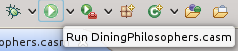
\includegraphics[scale=0.52] {images/run.png}
   \label{fig:runningASpec}
 }\quad
 \subfigure[\ldots by selecting its \emph{Run Configuration}]{
    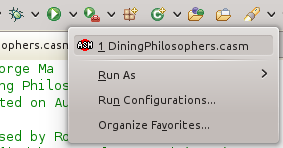
\includegraphics[scale=0.52] {images/run-by-configuration.png}
    \label{fig:run-by-config}
  }

\subfigure[The CoreASM menu]{
    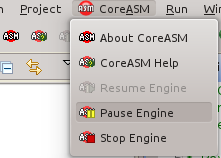
\includegraphics[scale=0.52] {images/coreasm-menu.png}
    \label{fig:coreasm-menu}
  }
   \quad\hspace{0.8cm}
 \subfigure[The output of the DiningPhilosophers specification]{
 	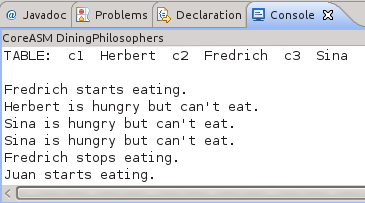
\includegraphics[scale=0.7] {images/output.png}
 	\label{fig:output}
 }
\caption{Running a CoreASM specification}
\label{fig:run}
\end{figure}
Running a specification the first time automatically creates a \emph{Run Configuration} which specifies some options for the execution of the related CoreASM specification. Fig.\,\ref{fig:run-config} on page\,\pageref{fig:run-config} shows the default \emph{Run Configuration} for the DiningPhilosophers specification. The different options for a certain specification configure the termination condition for a CoreASM execution and the verbosity of its output.

The second option to start a specification is to use a \emph{Run Configuration}. If a \emph{Run Configuration} for a specification exists, or after it has been created, its specification can be executed by selecting it. The down-arrow on the right-hand side of the \emph{Run}-button or the \emph{Run Configuration}-menu can be used to open a selection list (see fig.\,\ref{fig:run-by-config}). To access a \emph{Run Configuration} via the Eclipse menu, select \menu{\underline{R}un > Ru\underline{n} Configurations\ldots}.

\begin{figure}[h]
	\centering
	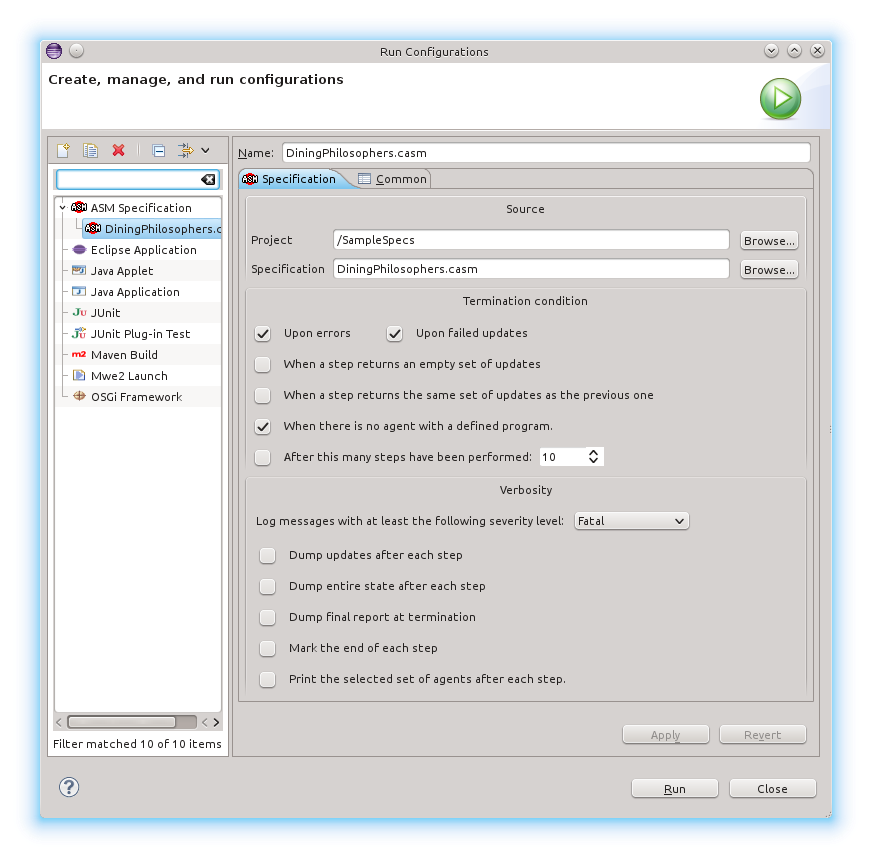
\includegraphics[width=0.8\textwidth]{images/run-configuration.png}
	\caption{Default \emph{Run Configuration} for the DiningPhilosophers specification}
	\label{fig:run-config}
\end{figure}

The execution of a specification can be paused, resumed, and stopped by clicking one of the buttons (see fig.\,\ref{fig:toolbar}) located under the CoreASM-menu or selecting an entry from that menu (see fig.\,\ref{fig:coreasm-menu}).

\section{Debugging a Specification}
A CoreASM specification can be started for debugging by either using the de\emph{bug}-button\,
\includegraphics[height=0.8em]{images/bug-icon.png} of the toolbar (see fig.\,\ref{fig:toolbar}) or by selecting a \emph{Debug Configuration} via the down-arrow beside this button. Another option is using the eclipse menu \menu{\underline{R}un>De\underline{b}ug Configurations\dots}.

If the specification has been paused by using one ot the pause-buttons 
\includegraphics[height=0.8em]{images/pause-button.png} 
\includegraphics[height=0.8em]{images/pause-button1.png}, or a break point has been reached, Eclipse asks the user to switch to the debug perspective. Confirming this question, the user will be shown a screen similar to fig.\,\ref{fig:debugger}. This debug perspective contains the views (from top left to bottom right) described in table\,\ref{table:debugger} on page\,\pageref{table:debugger}.

\begin{figure}[h]
\centering
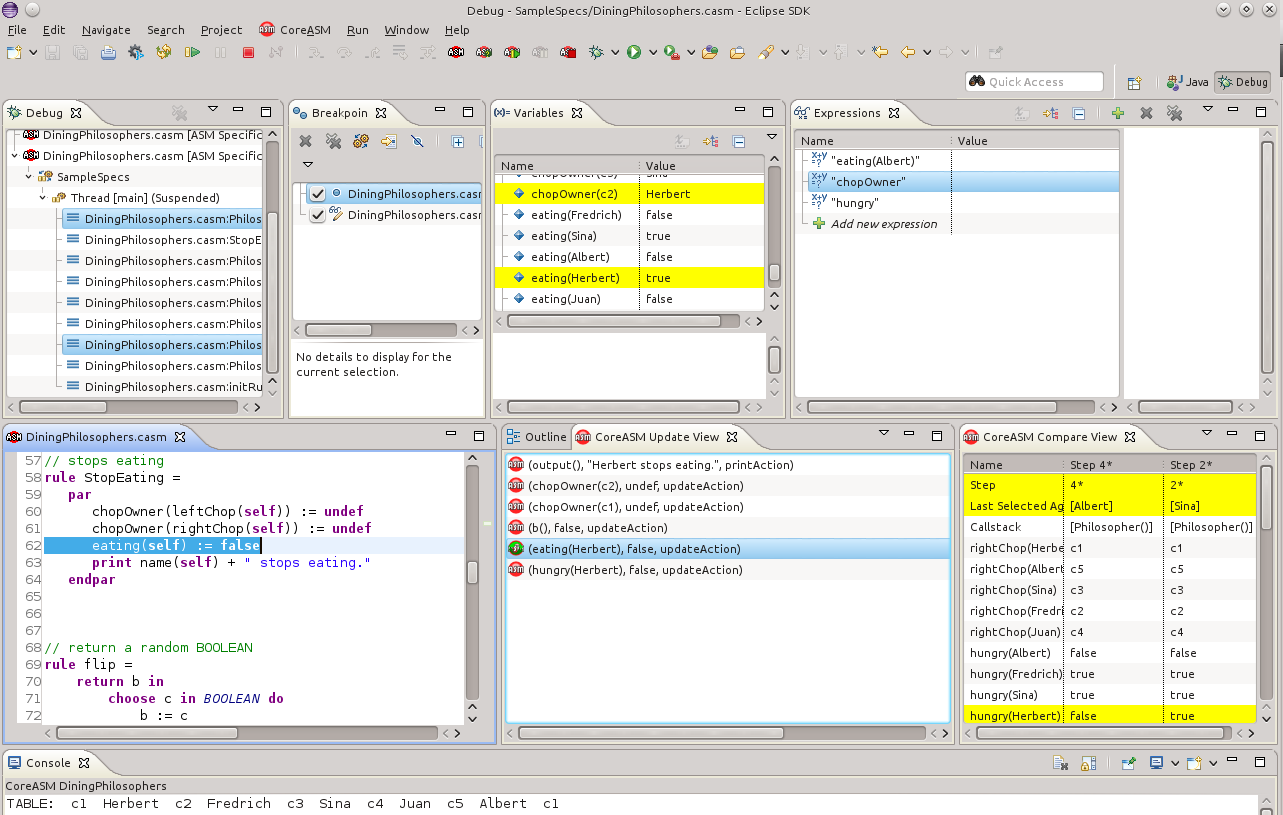
\includegraphics[width=.90\textwidth]{images/debugger-overview.png}
\caption{Overview of the Debugger}
\label{fig:debugger}
\end{figure}

\begin{table}[h]
\centering
\label{table:debugger}
\caption{Overview of the debugging components in fig.\,\ref{fig:debugger}}
	\begin{tabular}{|p{0.175\textwidth}|p{0.32\textwidth}|p{0.41\textwidth}|}
	\hline
	\textbf
	\textbf{View} & \textbf{Description} & \textbf{Interaction}\\
	\hline
	Debug & Shows the currently executed specification and its steps & Selected steps are taken into account for the CoreASM Compare View\\
	\hline
	Breakpoints & Lists all Breakpoints of the workspace & Breakpoint(s) can be disabled or re-enabled, skipped, deleted, exported, imported and used to navigate to its related source destination\\
	\hline
	Variables & Shows the state of the CoreASM engine & The state of the CoreASM execution can be investigated and manipulated\\
	\hline
	Expressions & Shows user defined CoreASM expressions and their values & User defined expressions are passed to the interpreter and evaluated based on the current state of the execution\\
	\hline
	Editor & Shows the statement to be evaluated next & Changes to the specification during debugging do not influence the current execution\\
	\hline
	Update View & Shows all updates, optionally restricted to a specific agent, which are collected up to now during the current step of the interpreter & An update can be used to navigate to the statement of its origin; Updates which correspond to a breakpoint are highlighted by a green symbol 
\includegraphics[height=0.8em]{images/breakpoint-update.png}.\\
	\hline
	Compare View & Shows the state of the CoreASM execution for specific steps & All selected steps in the \emph{Debug}-view are shown for comparison; Optionally, just differences are presented.\\
	\hline
	\end{tabular}
\end{table}
The debbuging of CoreASM specifications is described in detail in the following sections.

\subsection{Stepping Through a Specification}
Once the execution of a specification in debug mode is paused, one can analyze a specification step-by-step. There are three different kinds of stepping, which can be forced by pressing the related buttons 
\includegraphics[height=0.8em]{images/step-buttons.png} in the toolbar of the debug perspective or use a keyboard shortcut:
\begin{itemize}
	\item	
\includegraphics[height=0.8em]{images/step-return.png} | \keys{F7} Step Return\\
			Executing all statements and stopping at the next sequential block
	\item	
\includegraphics[height=0.8em]{images/step-over.png} | \keys{F6} Step Over\\
			Executing a single step of the machine
	\item 	
\includegraphics[height=0.8em]{images/step-in.png} | \keys{F5} Step Into\\
			Executing a single step, which can also be a step inside a sequential block
\end{itemize}
Debugging of imperative languages differs in many points from debugging Abstract State Machines. One difference is, that in a CoreASM specification without sequential parts, all different step actions result in collecting and aggregating all updates of the current step. The execution will stop again before the first statement of the next step will be computed, so that one can examine the update set before the state of the machine is updated.
To continue the execution of the interpreter click on one of the resume-buttons 
\includegraphics[height=0.8em]{images/resume-button.png} 
\includegraphics[height=0.8em]{images/resume-button1.png}.

\subsection{Adding/Removing Breakpoints}
A breakpoint can be set from within the source editor by double-clicking on the ruler or right-clicking it and selecting \menu{Toggle breakpoint} (see Fig.~\ref{fig:breakpoint-inside-editor}).

\begin{figure}[h]
\centering
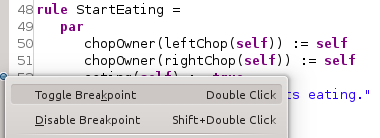
\includegraphics[scale=0.5]{images/line-breakpoint.png}
\caption{Line breakpoint set at line 52 of the DiningPhilosophers specification.}
\label{fig:breakpoint-inside-editor}
\end{figure}

There are three different types of breakpoints (see Fig.~\ref{fig:breakpoint-view}):
\begin{itemize}
  \item Watchpoints: They will be added if the selected line starts with
  ``function'' or ``universe''. They will suspend the execution whenever the value of a
  function/universe changes or is being read.
  \item Method breakpoints: They will be added if the selected line starts with
  \texttt{rule}. They will suspend whenever an update occurs from a line within the
  selected rule's body.
  \item Line breakpoints: They will be added if none of the above breakpoints can
  be added. They will suspend whenever an update occurs from the selected line.
\end{itemize}

\begin{figure}[h]
	\centering
	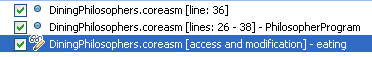
\includegraphics[scale=0.6]{images/debug-view-breakpoints.png}
	\caption{Three different kinds of breakpoints listed in the Breakpoints view.}
	\label{fig:breakpoint-view}
\end{figure}

A breakpoint can be disabled by choosing \menu{Toggle Breakpoint} from context menu of the ruler or by un-checking the box in front of its entry in the Breakpoints view. By enabling the \emph{Skip All Breakpoints}-toggle switch 
\includegraphics[height=0.8em]{images/skip-all-breakpoints.png}, all breakpoints are discounted during an execution without the need of changing the set of active breakpoints.

\subsection{Watching Functions and Expressions}
The \emph{Variables}-view (see Fig.~\ref{fig:variables-view}) allows to watch and examine the values of all available functions of the machine's state. All values that have been changed due to the last update-set are highlighted in yellow color. The value of a function at a specific location can be changed by clicking on its value entry, changing the value by modifying the text, and pressing \keys{\enter}. This modification is applied directly to the state of the machine and will not induce an extra update --- this feature has to be used with caution.

\begin{figure}[h]
\centering
	\subfigure[The \emph{Variables}-view shows all functions at its location, their value, definition type, and current type.]{
		\label{fig:variables-view}
		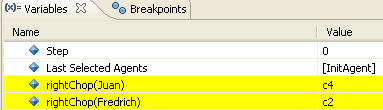
\includegraphics[scale=0.5]{images/variables-view.png}
	}
	\quad
	\subfigure[Context-menu of the \emph{Variables}-view.]{
		\label{fig:variables-view-popup-menu}
		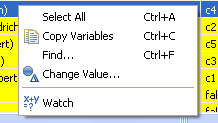
\includegraphics[scale=0.5]{images/variables-view-popup.png}
	}
\caption{The \emph{Variables}-view for inspecting function and modifying their values.}
\label{fig:collection-variables-view}
\end{figure}

To keep an eye on a specific function for a given location, a corresponding entry in the \emph{Expressions}-view (see fig.\,\ref{fig:function}) can be created by right-clicking on the desired entry and selecting \menu{Wa\underline{t}ch} from the menu (see Fig.~\ref{fig:variables-view-popup-menu}).
\begin{figure}[h]
\centering
	\subfigure[A function and its values for each location.]{
		\label{fig:function}
		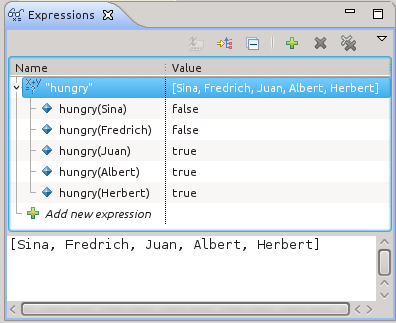
\includegraphics[scale=0.6]{images/expressions-view-function.png}
	}
	\quad
	\subfigure[Some functions of specific locations and their values. The marked entry shows a user defined expression and its value.]{
		\label{fig:functions-at-specific-locations}
		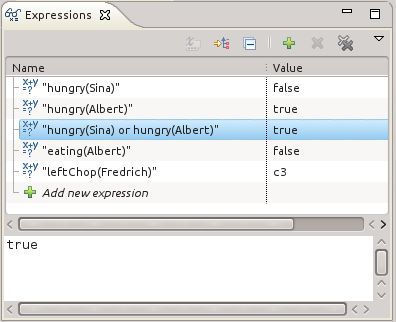
\includegraphics[scale=0.6]{images/expressions-view-for-locations.png}
	}

	\caption{The \emph{Expressions}-view shows user selected universes, functions for either all or one specific location, and evaluates user defined expressions depending on the current state.}
	\label{fig:expressions-view}
\end{figure}

Additional expressions can be added to the \emph{Expressions}-view by pressing 
\includegraphics[height=0.8em]{images/add-new-expression.png} and entering either a universe name, or function name and its location (see fig.\,\ref{fig:functions-at-specific-locations}). Entering a function name without its location (e.g. hungry) will result in showing a container of all it's locations and values (see Fig.~\ref{fig:function}).
Expressions can be removed by selecting at least one entry and pressing \keys{\del}, or using the buttons 
\includegraphics[height=0.8em]{images/expression-remove.png}.


Another way to inspect expressions on the fly is marking an expression inside the \emph{Editor}-view or moving the mouse over a single statement. By doing so, a tooltip will be presented that shows the result of the evaluation of the marked expression based on the current context of the machine's evaluation, i.\,e. the global state and the current computation context. Two examples are given in fig.\,\ref{fig:on-the-fly}.

\begin{figure}[h]
\centering
	\subfigure[The expression at the line breakpoint is evaluated on-the-fly.]{
		\label{fig:on-the-fly-evaluation}
		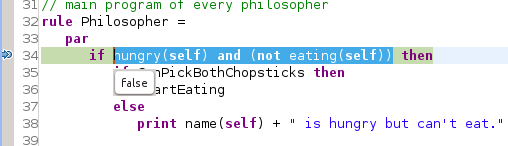
\includegraphics[scale=0.45]{images/on-the-fly-evaluation.png}
	}
	\quad
	\subfigure[The result of the derived function \texttt{CanPickBothChopsticks} is presented as a tooltip when the mouse cursor hovers over its calling statement.]{
		\label{fig:on-the-fly-evaluation-single-exp}
		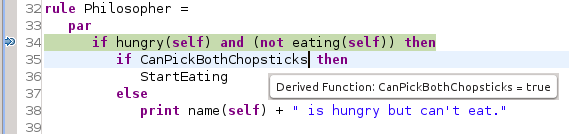
\includegraphics[scale=0.45]{images/on-the-fly-evaluation-single-exp.png}
	}

	\caption{During debugging, expressions can be marked inside the \emph{Editor}-view so that the result will be shown as a tooltip.}
	\label{fig:on-the-fly}
\end{figure}

\section{Taking Care of Updates}
The \emph{Update}-view (see fig.\,\ref{fig:update-view-and-source}) lists all updates which have been computed during the current step. Each update is a triple, consisting of the function and its location, the value, and the type of action. The action type is an internal CoreASM specific value. By double-clicking on an update-entry, the source of this update inside the specification is presented to the user. Updates that correspond to an active breakpoint are marked by a green symbol 
\includegraphics[height=0.8em]{images/breakpoint-update.png}. To focus on the updates of a specific agent, a filter option can be applied (see fig.\,\ref{fig:filter-update-view}).

\begin{figure}[h]
	\centering
	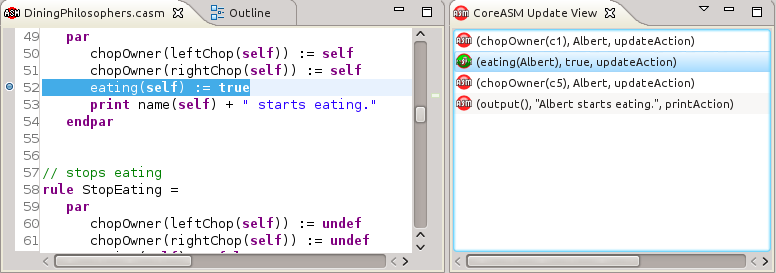
\includegraphics[scale=0.65]{images/update-view-with-source.png}
	\caption{The \emph{Editor} (left) and \emph{Update}-view (right): The statement in the specification causing the marked update is highlighted. It is located in a line with an active breakpoint.}
	\label{fig:update-view-and-source}
\end{figure}

\section{What has been changed?}
The \emph{Compare}-view enables analyzing the state of the machine over the time. Therefore, the view shows all functions and their values for selected steps of the machine side-by-side. The selection has to be performed within the \emph{Breakpoints}-view where all steps are listed. Multiple steps can be selected while holding \keys{\ctrl} (for single selection) or holding \keys{\shift} (to mark a range of steps). Steps, which are marked by a $^*$ are intermediate steps resulting from sequential steps. To clear up the \emph{Compare}-view the filter option can be used, which results in hiding all corresponding functions with equal values (see fig.\,\ref{fig:filter-compare-view}, p.\,\pageref{fig:filter-compare-view}).

\begin{figure}[h]
\centering
	\subfigure[The filter of the \emph{Update}-view helps the user to concentrate on the updates of a specific agent.]{
		\label{fig:filter-update-view}
		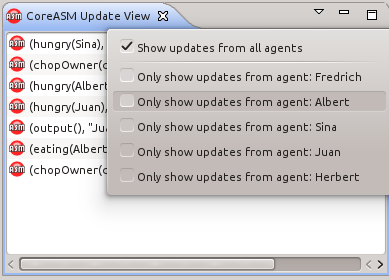
\includegraphics[scale=0.63]{images/filter-update-view.png}
	}
	\quad
	\subfigure[The \emph{Compare}-view shows the functions for different states side-by-side. To focus on the changes between those states, the filter can be used to hide functions with equal values.]{
		\label{fig:filter-compare-view}
		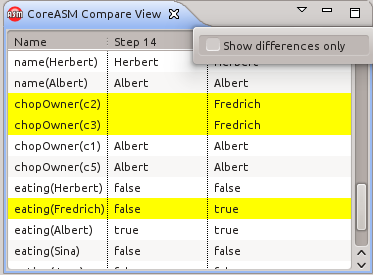
\includegraphics[scale=0.63]{images/filter-compareview.png}
	}

	\caption{Both, the \emph{Update}- and the \emph{Compare}-view offer filters to focus on certain aspects.}
	\label{fig:filters}
\end{figure}

\section{Excursus --- Modules in CoreASM: Hello World}\label{ch:hello-world}
The following specification \mydirectory{HelloWorld.casm} implements an extended ``Hello World!''. This specification itself specifies the output of ``we proudly present:''. It further demonstrates the use of modules by including the module \mydirectory{PrintHelloWorld.casm} which implements the output of ``Hello World!''. As a result, the rule \texttt{PrintHelloWorld} can be called from the initial rule of the main specification ``HelloWorld''.
\begin{lstlisting}
/** A multi-line comment
*   for the HelloWorld specification
*   Each specification has to start with CoreASM <name>
*/
CoreASM HelloWorld

//A single line comment previous to the block of used plugins
use Standard
use Modularity

//the initial rule definition
init HelloWorld

/** The path to an included CoreASM module
*   has to be given within double quotes.
*/
include "./PrintHelloWorld.casm"

rule HelloWorld =
seq
	print "we proudly present:"
next
	PrintHelloWorld()
\end{lstlisting}
The module \mydirectory{PrintHelloWorld.casm} implements the output of ``Hello World!''. In difference to a main specification, its header starts with \texttt{CoreModule <module name>} and an init rule is not allowed here.
\begin{lstlisting}
//modules can be included in CoreASM specifications
CoreModule PrintHelloWorld

use Standard

rule PrintHelloWorld =
	print "Hello World!"
\end{lstlisting}

Further example specifications, e.\,g. the DiningPhilosophers specification, are part of the distributable and can be found in the folder \mydirectory{sampleSpecs}.

\phantomsection
\addcontentsline{toc}{section}{References}
\bibliography{CoreASM_Eclipse_Debugger_Manual}
\bibliographystyle{plain}
\end{document}
